\documentclass[thesis.tex]{subfiles}              


\externaldocument[C2-]{chapter02}

\begin{document}

\chapter{Introduction}
%-----------------------------------------------------------
%Explain the aims and rationale for the physics case and what you have done. At the end of the introduction you should give a brief summary of the structure of the report. Motivate the reader and give overarching ideas. Describe what has been done and the structure of the report (how is it organized).

%\subsection{Background and Motivation}

In this project we aim to design and develop a system for analyzing medical videos from a camera pill, as seen in Figure \ref{fig:pill-cam}. The pill is swallowed and records video of the entire digestive system The goal is to be able to detect different irregularities in the patients digestive system, like a colon polyp, Chron's disease, Colorectal cancer, etc. by using video object tracking, object detection, machine learning or other relevant tools.

Neural networks models that we would like to explore further for this purpose are Convolutional neural networks (CNN), Recurrent neural networks (RNN), Capsule neural networks, Long Short-Term memory networks and more.

The main idea is to go beyond image-based methods and also exploit the time factor of the data. 
The videos we will be using for this is delivered by Bærum Hospital, and is carefully labeled by using tools such as described in the paper \citetitle*{ExpertDriven15}. In this paper \citeauthor*{ExpertDriven15} presents a semi-supervised method to gather the annotations in a easy and time saving way \cite{ExpertDriven15}. 

\begin{figure}[H] % pill-cam
  \begin{center}
    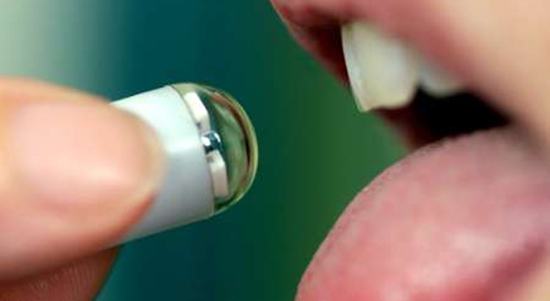
\includegraphics[width=\linewidth]{pill-cam.jpg}
    \caption{Illustration of how such a camera pill could look like \cite{PillCamCamera}.}
    \label{fig:pill-cam}
  \end{center}
\end{figure}

Colorectal cancer (CRC) is the third most common cause of cancer mortality for both men and women \cite{CancerStatistics10}, and it is a condition where early detection is of clear value for the ultimate survival of the patient. As statistics show that 15\% of male and female above 50 years are at risk, the procedure is recommended on a regular basis (every 3-5 years) for the population over 50, and from an earlier age for high-risk groups. Colonoscopy is a demanding procedure requiring an significant amount of time by specialized physicians, in addition to the discomfort and risks inherent in the procedure. Traditional methods based on colonoscopy are not cost-effective for population-based screening purposes, so only about 2-3\% of the target population is reached at present. The cost of a population screening program is prohibitively expensive. Colonoscopy is the most expensive cancer screening process in the US, with annual costs of \$10 billion dollars (\$1100 per person). In Norway we have similar costs of around \$1000 per person, with a time consumption of about 1 doctor-hour and 2 nurse-hours per examination. By researching an automatic system for a camera pill the aim is to greatly increase the number of patients that can be examined, i.e., making the public health care system more scalable and cost effective, while at the same time reducing the need for intrusive procedures like "bottom-up" examinations like colonoscopy.

%\subsection{Problem statement}


\end{document}